\documentclass[12pt]{article}
\usepackage{tikz}
\usetikzlibrary{positioning}


% Define macros
\newcommand\pgfmathsinandcos[3]{%
  \pgfmathsetmacro#1{sin(#3)}%
  \pgfmathsetmacro#2{cos(#3)}%
}

\newcommand\LongitudePlane[3][current plane]{
  \pgfmathsinandcos\sinEl\cosEl{#2} % elevation
  \pgfmathsinandcos\sint\cost{#3} % azimuth
  \tikzset{#1/.estyle={cm={\cost,\sint*\sinEl,0,\cosEl,(0,0)}}}
}

\newcommand\LatitudePlane[3][current plane]{%
  \pgfmathsinandcos\sinEl\cosEl{#2} % elevation
  \pgfmathsinandcos\sint\cost{#3} % latitude
  \pgfmathsetmacro\yshift{\cosEl*\sint}
  \tikzset{#1/.estyle={cm={\cost,0,0,\cost*\sinEl,(0,\yshift)}}} %
}

\newcommand\DrawLongitudeCircle[2][1]{
  \LongitudePlane{\angEl}{#2}
  \tikzset{current plane/.prefix style={scale=#1}}
  \pgfmathsetmacro\angVis{atan(sin(#2)*cos(\angEl)/sin(\angEl))} %
  \draw[current plane,thin] (\angVis:1) arc (\angVis:\angVis+180:1);
  \draw[current plane,thin,dashed] (\angVis-180:1) arc (\angVis-180:\angVis:1);
}

\newcommand\DrawLongitudeCircleBlue[2][1]{
  \LongitudePlane{\angEl}{#2}
  \tikzset{current plane/.prefix style={scale=#1}}
  \pgfmathsetmacro\angVis{atan(sin(#2)*cos(\angEl)/sin(\angEl))} %
  \draw[current plane,thin,blue] (\angVis:1) arc (\angVis:\angVis+180:1);
  \draw[current plane,thin,dashed,blue] (\angVis-180:1) arc (\angVis-180:\angVis:1);
}

\newcommand\DrawLatitudeCircle[2][1]{
  \LatitudePlane{\angEl}{#2}
  \tikzset{current plane/.prefix style={scale=#1}}
  \pgfmathsetmacro\sinVis{sin(#2)/cos(#2)*sin(\angEl)/cos(\angEl)}
  \pgfmathsetmacro\angVis{asin(min(1,max(\sinVis,-1)))}
  \draw[current plane,thin,black] (\angVis:1) arc (\angVis:-\angVis-180:1);
  \draw[current plane,thin,dashed] (180-\angVis:1) arc (180-\angVis:\angVis:1);
}

\newcommand\DrawLatitudeCircleRed[2][1]{
  \LatitudePlane{\angEl}{#2}
  \tikzset{current plane/.prefix style={scale=#1}}
  \pgfmathsetmacro\sinVis{sin(#2)/cos(#2)*sin(\angEl)/cos(\angEl)}
  \pgfmathsetmacro\angVis{asin(min(1,max(\sinVis,-1)))}
  \draw[current plane,thin,red] (\angVis:1) arc (\angVis:-\angVis-180:1);
  \draw[current plane,thin,dashed,red] (180-\angVis:1) arc (180-\angVis:\angVis:1);
}


\tikzset{
  >=latex,
  inner sep=0pt,
  outer sep=2pt,
  mark coordinate/.style={inner sep=0pt,outer sep=0pt,minimum size=3pt,
    fill=black,circle}
}

\usepackage{amsmath}
\usetikzlibrary{arrows}
\pagestyle{empty}
\usepackage{pgfplots}
\usetikzlibrary{calc,fadings,decorations.pathreplacing}

\begin{document}

	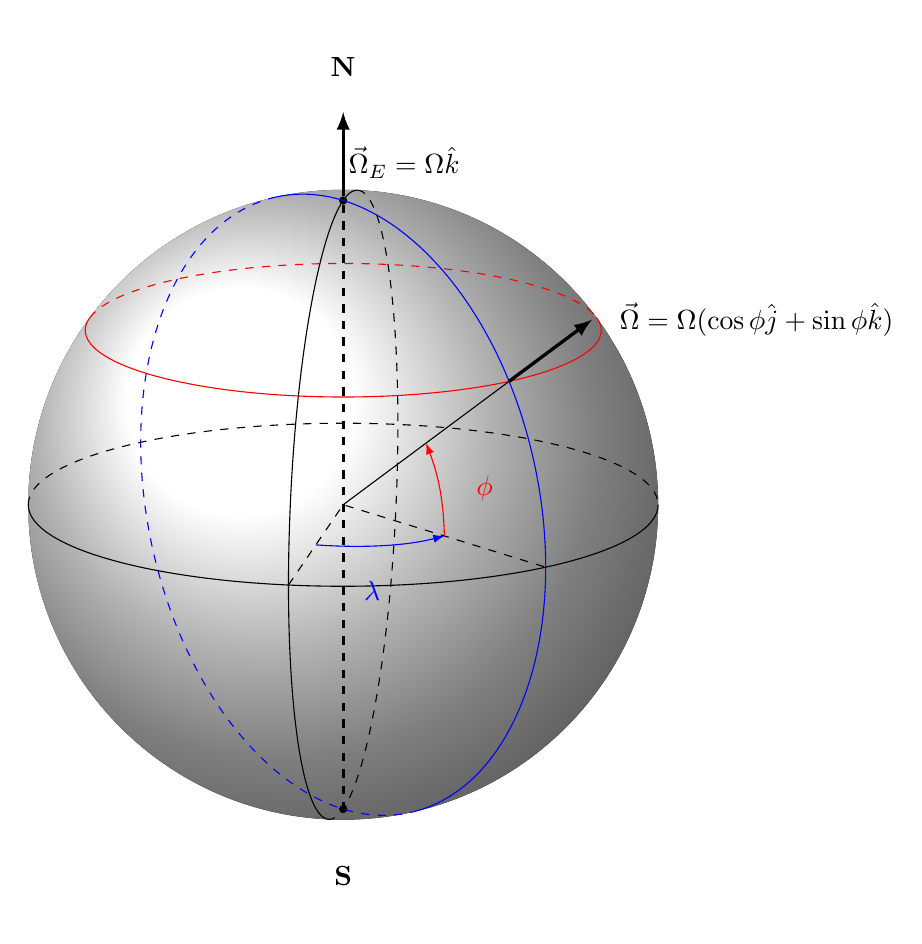
\begin{tikzpicture}[scale=1,every node/.style={minimum size=1cm}]


	% Define some variables
	\def\R{4}                   % sphere radius
	\def\angEl{15}           % elevation angle
	\def\angAz{-100}      % azimuth angle
	\def\angPhiOne{-50} % longitude of point P
	\def\angBeta{35}      % latitude of point P and Q
		
	\pgfmathsetmacro\H{\R*cos(\angEl)}
	\LongitudePlane[xzplane]{\angEl}{\angAz}
	\LongitudePlane[pzplane]{\angEl}{\angPhiOne}
	\LatitudePlane[equator]{\angEl}{0}
	\fill[ball color=white!10] (0,0) circle (\R); % 3D lighting effect
	\coordinate (O) at (0,0);
	\coordinate[mark coordinate] (N) at (0,\H);
	\coordinate[mark coordinate] (S) at (0,-\H);
	\path[xzplane] (\R,0) coordinate (XE);
	
	\path[pzplane] (\angBeta:\R) coordinate (P);
	\path[pzplane] (\angBeta:\R+2) coordinate (Pd);
	\path[pzplane] (\R,0) coordinate (PE);
    	\path[pzplane] (\R+4,0) coordinate (PEd);

    	\DrawLongitudeCircle[\R]{\angAz}
    	\DrawLongitudeCircleBlue[\R]{\angPhiOne}
    	\DrawLatitudeCircleRed[\R]{\angBeta}
	\DrawLatitudeCircle[\R]{0} 

	\node[above=32pt] (Nabove) at (N) {$\mathbf{N}$};
	\node[below=8pt] (Sbelow) at (S) {$\mathbf{S}$};
	
	\draw[-,dashed, very thick] (N) -- (S);
	\draw[->,very thick] (N) -- node[pos=0.4,right] {$\vec{\Omega}_E = \Omega \hat k$} (Nabove);
	\draw[-] (O) -- (P);
	\draw[dashed] (XE) -- (O) -- (PE);
	\draw[->,black,very thick] (P) -- node[pos=1.0,right=8pt] {$\vec{\Omega} = \Omega ( \cos \phi \hat j + \sin \phi \hat k )$} (Pd);
    		
	\draw[pzplane,->,thin,red] (0:0.5*\R) to[bend right=15]
	    node[midway,right] {$\phi$} (\angBeta:0.5*\R);
	\draw[equator,->,thin,blue] (\angAz:0.5*\R) to[bend right=30]
	    node[pos=0.4,below] {$\lambda$} (\angPhiOne:0.5*\R);
    	
	\end{tikzpicture}

\end{document} 